\documentclass[tikz,border=3pt]{standalone}

\definecolor{juliagreen}{HTML}{389826}
\definecolor{juliared}{HTML}{CB3C33}
\definecolor{juliapurple}{HTML}{9558B2}
\definecolor{juliablue}{HTML}{4063d8}

\begin{document}
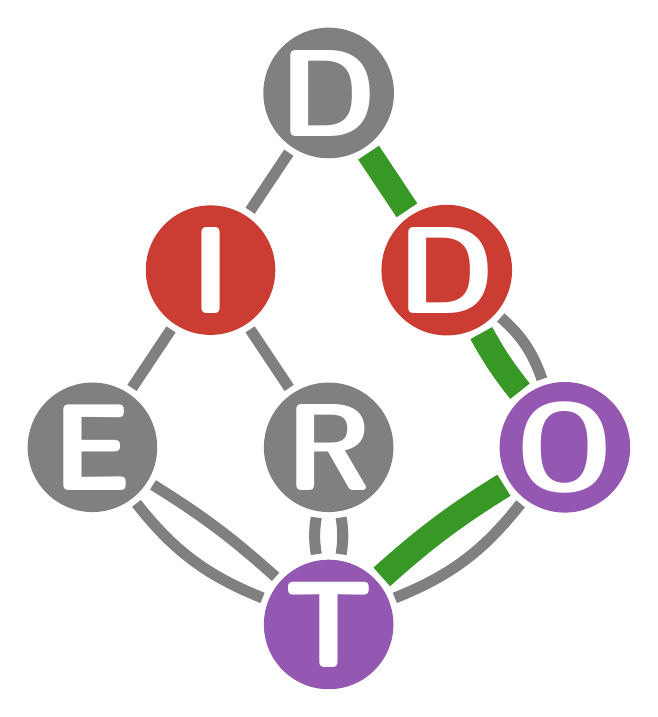
\begin{tikzpicture}[scale=1.5]
  \tikzstyle{o} = [circle, color=white, fill=black!50,
  inner sep=0pt, minimum width={26pt}, align=center, scale=1.8,
  font=\fontfamily{cmss}\Huge\selectfont];
  \tikzstyle{b} = [fill=juliared];
  \tikzstyle{a} = [line width=4pt, shorten <=2pt, shorten >=2pt, color=black!50];
  \tikzstyle{p} = [line width=9pt, color=juliagreen];

  \node[o] (r) at (2, 4.5) {\textbf{D}};

  \node[o,b] (1a) at (1, 3) {\textbf{I}};
  \node[o,b] (1b) at (3, 3) {\textbf{D}};

  \node[o] (2a) at (0, 1.5) {\textbf{E}};
  \node[o] (2b) at (2, 1.5) {\textbf{R}};
  \node[o,fill=juliapurple] (2c) at (4, 1.5) {\textbf{O}};

  \node[o,fill=juliapurple] (t) at (2, 0) {\textbf{T}};

  \draw[a] (r) to (1a);
  \draw[a,p] (r) to (1b);

  \draw[a] (1a) to (2a);
  \draw[a] (1a) to (2b);
  \draw[a] (1b) to[bend left=15] (2c);
  \draw[a,p] (1b) to[bend right=5] (2c);

  \draw[a] (2a) to[bend right=15] (t);
  \draw[a] (2a) to[bend left=5] (t);
  \draw[a] (2b) to[bend right=10] (t);
  \draw[a] (2b) to[bend left=10] (t);
  \draw[a,p] (2c) to[bend right=5] (t);
  \draw[a] (2c) to[bend left=15] (t);
\end{tikzpicture}
\end{document}
